\documentclass[12pt]{book}
\usepackage[margin=.85in]{geometry} % for MARGIN
\usepackage[many]{tcolorbox}    	% for COLORED BOXES (tikz and xcolor included)


\usepackage{multicol}   
\usepackage{enumerate}
\usepackage[shortlabels]{enumitem}
\usepackage{varwidth}
\usepackage{tasks}
\usepackage[export]{adjustbox}

\usepackage{titleps}
\usepackage{setspace}               % for LINE SPACING
\usepackage[⟨options⟩]{fancyhdr}
\usepackage{enumitem}
\setlist{nosep}
\usepackage{tikz}
\usepackage{pgfplots}
\pgfplotsset{compat=1.5.1}
\usetikzlibrary{datavisualization}
\usetikzlibrary{datavisualization.formats.functions}

\newcommand{\D}{\displaystyle}


\setlength\parindent{0pt}   % killing indentation for all the text
\setstretch{1.3}            % setting line spacing to 1.3
\setlength\columnsep{0.25in} % setting length of column separator
\pagestyle{fancy}           % setting pagestyle to be headings

\usepackage[]{titlesec}

\fancyhead[L]{Math V04 - College Algebra}
\fancyhead[R]{Christina Papazacharioudakis}

\tcbset{
    sharp corners,
    colback = white,
    before skip = 0.2cm,    % add extra space before the box
    after skip = 0.5cm      % add extra space after the box
}                           % setting global options for tcolorbox

    \newtcolorbox{boxR}{
    fontupper = \color{black}, % font color
    boxrule = 1.5pt,
    colframe = black,
    rounded corners,
    arc = 5pt   % corners roundness
}

\definecolor{ballblue}{rgb}{0.13, 0.67, 0.8}

\begin{document}



\begin{comment}
Name: \underline{\hspace{100mm}}
\vspace{20mm}
  \centerline{\Large \textbf{Chapter 2: Equations and Inequalities} } 

{\large
\begin{center}
\begin{varwidth}{\textwidth}
\begin{enumerate}[2.1]
    \item The Regular Coordinate System and Graphs
    \item Linear Equations in One Variable
    \item Models and  Applications (Skipping)
    \item Complex Numbers
    \item Quadratic Equations
    \item Other Types of Equations
    \item Linear Inequalities and Absolute Value Inequalities
\end{enumerate}
\end{varwidth}
\end{center}

}
\newpage  
\end{comment}

{\Large \textbf{6.3 \& 6.4 Logarithmic Functions Functions and Their Graphs}}

In these two sections, our focus is on studying the \textbf{inverse of the exponential function}, called the \textbf{logarithmic function}. Since the logarithmic function is an inverse function, let's review some concepts on inverse functions:


\centerline{\includegraphics[scale=0.6]{Chapter 6/6.3-figure1.png}}
\vspace{3mm}

{\large \textbf{The Definition of a Logarithmic Function}}

Looking at the graph of an exponential function, is it one-to-one? 


\begin{multicols}{2}
$b>1$:

    \begin{tikzpicture}[scale=0.7, transform shape]
\begin{axis}[
    ymin=-1.5,
    ymax=10.5,
    xmin=-5.5,
    xmax=5.5,
    axis on top=true,
    axis x line=middle,
    axis y line=middle,
    axis line style={latex-latex},
    xlabel=$x$,
    ylabel=$y$,
    xticklabels=\empty,
    yticklabels=\empty,
    xtick distance=1,
    ytick distance=1,
 %  xmajorgrids=true,
%   ymajorgrids=true,
  axis equal = true, 
    every axis x label/.style={at={(ticklabel* cs:1.0)}, anchor=west,},
    every axis y label/.style={at={(ticklabel* cs:1.0)}, anchor=south,}
]
 \pgfplotsset{ticks=none}
    \addplot [<->][very thick, samples=100, domain=-5:3.4] {2^x};
    \addplot[dashed, thick, domain=-9:9,red] ({x},0.01);
\end{axis}
\end{tikzpicture}

$b<1$:

\begin{tikzpicture}[scale=0.7, transform shape]
\begin{axis}[
    ymin=-1.5,
    ymax=10.5,
    xmin=-5.5,
    xmax=5.5,
    axis on top=true,
    axis x line=middle,
    axis y line=middle,
    axis line style={latex-latex},
    xlabel=$x$,
    ylabel=$y$,
    xticklabels=\empty,
    yticklabels=\empty,
    xtick distance=1,
    ytick distance=1,
 %  xmajorgrids=true,
%   ymajorgrids=true,
  axis equal = true, 
    every axis x label/.style={at={(ticklabel* cs:1.0)}, anchor=west,},
    every axis y label/.style={at={(ticklabel* cs:1.0)}, anchor=south,}
]
 \pgfplotsset{ticks=none}
    \addplot [<->][very thick, samples=100, domain=-3.4:5] {2^(-x)};
    \addplot[dashed, thick, domain=-9:9,red] ({x},0.01);
\end{axis}
\end{tikzpicture}
\end{multicols}

Does $f(x)=b^x$ have an inverse function?

\newpage

Since $f(x)=b^x$ passes the horizontal line test, it is a one-to-one function and therefore has an inverse. Let us use the four-step process to find the inverse: 


\vspace{80mm}





\begin{boxR}
    \textbf{Definition of a Logarithmic Function}
    \vspace{1mm}
    \hline
    \vspace{2mm}
    For $x>0$ and $b>0 \hspace{2mm} (b \neq1)$, 

    $$y=\log_bx \text{ is equivalent to } b^y=x$$

    The function $f(x)=\log_bx$ is the \textbf{logarithmic function function with base b.}
\end{boxR}


\vspace{10mm}
The equations $$ y=\log_bx \text{\hspace{4mm} and \hspace{4mm} } b^y=x $$ 

are different ways of expressing the same thing.
\newpage

\centerline{\includegraphics[scale=.6]{Chapter 6/6.3-figure2.png}}
\vspace{5mm}

\underline{\textbf{Example 1 - Converting from Logarithmic Form to Exponential Form}}

Write the following logarithmic equations in exponential form.
\vspace{2mm}
\begin{enumerate}[(a)]
    \item $\D \log_6 (\sqrt{6})=\frac{1}{2}$
    \vspace{25mm}
    \item $\D \log_3 (9)=2$
    \vspace{25mm}
    \item $\D \log_5(x)=2$
    \vspace{25mm}
    \item $\D \log_3(7)=y$
    \vspace{25mm}    
\end{enumerate}

There is a visual ``spiral'' pattern you can use when going from Logarithmic Form to Exponential Form:



\newpage
Now we work on going the other direction between forms. We will start with the exponential form of an equation and convert it to logarithmic form. 

As a reminder,  $$ y=\log_bx \text{\hspace{4mm} is the same as \hspace{4mm} } b^y=x $$ 

\vspace{5mm}

\underline{\textbf{Example 2 - Converting from Exponential Form to Logarithmic Form}}

Write the following exponential equations in logarithmic form.
\vspace{2mm}
\begin{enumerate}[(a)]
    \item $\D 2^3=8$
    \vspace{30mm}
    \item $ \D 10^{-4} = \frac{1}{10000}$
    \vspace{30mm}
    \item $12^2=x$
    \vspace{30mm}
    \item $e^y=9$
\end{enumerate}
\newpage


{\large \textbf{Evaluating Logarithms}}

Knowing the squares, cubes, and roots of numbers allows us to evaluate logarithms. For example, consider $$\log_4(16)$$ We ask ourselves, ``$4$ to what power gives me 16?"

\vspace{10mm}


\underline{\textbf{Example 3 - Evaluating Logarithms}}

Evaluate: 
\begin{enumerate}[(a)]
    \item $\D \log_2(16)$
    \vspace{3mm}
    \item $\D \log_7\left(\frac{1}{49}\right)$
    \vspace{3mm}
    \item $\D \log_{25}(5)$
    \vspace{3mm}
    \item $\D \log_2(\sqrt[5]{2})$
\end{enumerate}
\vspace{50mm}


\newpage
{\large \textbf{Basic Logarithmic Properties}}

Because logarithms are exponents, they have properties that can be verified using properties of exponents.
\vspace{1mm}

\begin{boxR}
    \textbf{Basic Logarithmic Properties Involving One}
    \vspace{1mm}
    \hline
    \vspace{2mm}
    \begin{enumerate}
        \item $\D\log_b(b)=1$
        \vspace{1mm}
        \item $\D \log_b(1)=0$
    \end{enumerate}
\end{boxR}
\vspace{3mm}

\underline{\textbf{Example 4 - Using Properties of Logarithms}}

Evaluate:

\begin{enumerate}
    \item $\log_7(7)$
    \vspace{5mm}
    \item $\log_5(1)$
    \vspace{5mm}
\end{enumerate}


Now that we are familiar with logarithmic notation, let's revisit solving the inverse of $f(x)=b^x$.

\begin{enumerate}[\textbf{Step} 1:]
    \item Replace $f(x)$ with $y$:
    \vspace{10mm}
    \item Swap $x$ and $y$:
    \vspace{10mm}
    \item Solve for $y$:
    \vspace{10mm}
    \item Replace $y$ with $f^{-1}(x)$:
    \vspace{10mm}
\end{enumerate}

Recall from Section 3.7 we learned that: 
$$ f(f^-1(x))=x \text{ and } f^{-1}(f(x))=x$$

\newpage
We now have the following \textbf{inverse properties of logarithms}:
\vspace{1mm}

\centerline{\includegraphics[scale=.7]{Chapter 6/6.3-figure3.png}}


\underline{\textbf{Example 5 - Using Inverse Properties of Logarithms}}

Evaluate:
\begin{enumerate}[(a)]
    \item $\D \log_44^5$
    \vspace{1mm}
    \item $\D 6^{\log_6 9}$
\end{enumerate}
\vspace{5mm}

{\large \textbf{Graphs of Exponential and Logarithmic Functions}}
\vspace{1mm}

How do we graph exponential functions? We use the fact that a logarithmic function is the inverse of an exponential function. This means that the logarithmic function reverses the coordinates of the exponential function. Reversing the coordinates creates a reflection of the graph of the exponential function about the line $y=x$.
\vspace{5mm}



\underline{\textbf{Example 6 - Graphs of Exponential and Logarithmic Functions}}

Graph $f(x)=2^x$ and $g(x)=\log_2(x)$ in the same rectangular coordinate system.
\vspace{2mm}

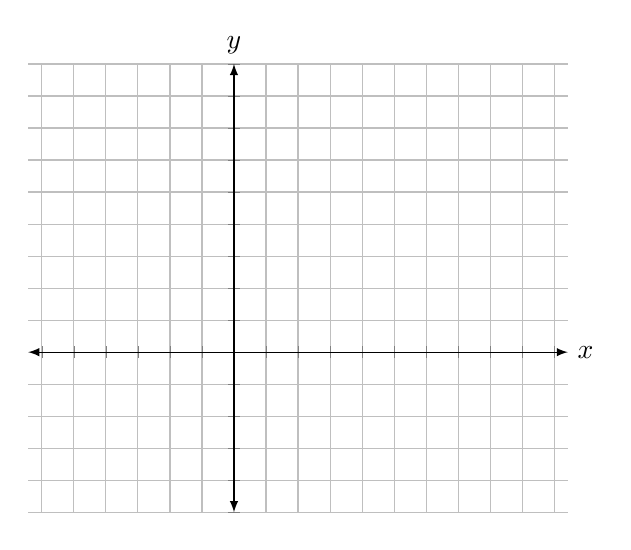
\begin{tikzpicture}[scale=1, transform shape]
\begin{axis}[
    ymin=-5,
    ymax=9,
    xmin=-5,
    xmax=9,
    axis on top=true,
    axis x line=middle,
    axis y line=middle,
    axis line style={latex-latex},
   % minor tick num=1,
   % major tick num=5,
    xlabel=$x$,
    ylabel=$y$,
   xticklabels=\empty,
  yticklabels=\empty,
   xtick distance=1,
    ytick distance=1,
  xmajorgrids=true,
 ymajorgrids=true,
     axis equal = true, 
    every axis x label/.style={at={(ticklabel* cs:1.0)}, anchor=west,},
    every axis y label/.style={at={(ticklabel* cs:1.0)}, anchor=south,}
]
   

\end{axis}
\end{tikzpicture} 


\newpage




\newpage
Depending if $b$ is less than $1$ or greater than $1$, we have the following graphs of exponential and logarithmic functions. 
\vspace{5mm}

\centerline{\includegraphics[scale=.7]{Chapter 6/6.3-figure4.png}}
The graphs in red illustrate the following general characteristics of logarithmic functions: 
\vspace{5mm}

\centerline{\includegraphics[scale=.7]{Chapter 6/6.3-figure5.png}}

\vspace{5mm}




\newpage
{\large \textbf{Graphing Logarithmic Functions}}

Let us again look at the graph of $g(x)=\log_2(x)$: 

\centerline{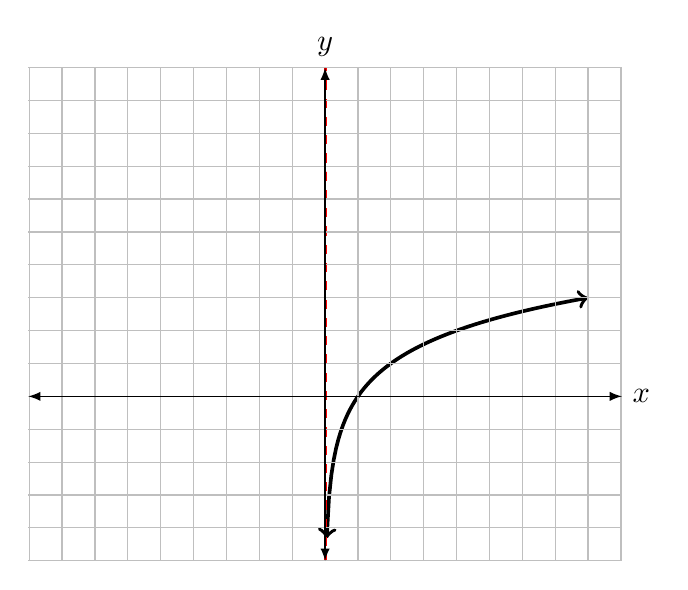
\begin{tikzpicture}[scale=1.1, transform shape]
\begin{axis}[
    ymin=-5,
    ymax=10,
    xmin=-5,
    xmax=5,
    axis on top=true,
    axis x line=middle,
    axis y line=middle,
    axis line style={latex-latex},
   % minor tick num=1,
   % major tick num=5,
    xlabel=$x$,
    ylabel=$y$,
   xticklabels=\empty,
  yticklabels=\empty,
   xtick distance=1,
    ytick distance=1,
  xmajorgrids=true,
 ymajorgrids=true,
     axis equal = true, 
    every axis x label/.style={at={(ticklabel* cs:1.0)}, anchor=west,},
    every axis y label/.style={at={(ticklabel* cs:1.0)}, anchor=south,}
]
    \pgfplotsset{ticks=none}
    \addplot [<->][very thick, samples=200, domain=-6:8] {log2(x)};
     \addplot[dashed, thick, domain=-9:10,red] (0.01,{x});
\end{axis}
\end{tikzpicture} }

How can we graph $f(x)=\log_2(x+1)$ and $h(x)=-\log_2(x)+2$ above  without making a table? 

\vspace{30mm}
\centerline{\includegraphics[scale=.63]{Chapter 6/6.3-figure6.png}}
\newpage

{\large \textbf{The Domain of a Logarithmic Function}}

Looking back at our graph of $f(x)=\log_2(x+1)$. 

\centerline{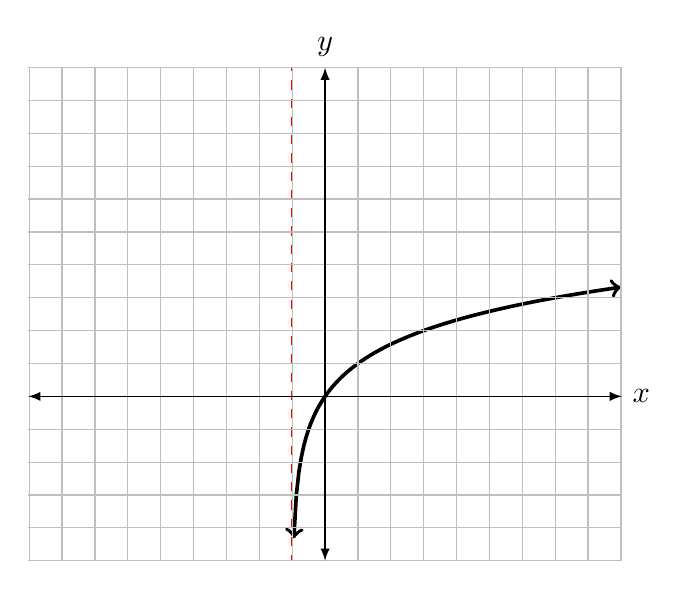
\begin{tikzpicture}[scale=1.1, transform shape]
\begin{axis}[
    ymin=-5,
    ymax=10,
    xmin=-5,
    xmax=5,
    axis on top=true,
    axis x line=middle,
    axis y line=middle,
    axis line style={latex-latex},
   % minor tick num=1,
   % major tick num=5,
    xlabel=$x$,
    ylabel=$y$,
   xticklabels=\empty,
  yticklabels=\empty,
   xtick distance=1,
    ytick distance=1,
  xmajorgrids=true,
 ymajorgrids=true,
     axis equal = true, 
    every axis x label/.style={at={(ticklabel* cs:1.0)}, anchor=west,},
    every axis y label/.style={at={(ticklabel* cs:1.0)}, anchor=south,}
]
    \pgfplotsset{ticks=none}
    \addplot [<->][very thick, samples=200, domain=-6:9] {log2(x+1)};
    \addplot[dashed, thick, domain=-9:10,red] (-.999,{x});
\end{axis}
\end{tikzpicture} }

Visually, is the domain of $f(x)$? 
\vspace{15mm}

In practice, to find the domain computationally, we take the input of the logarithmic function, and force it to be strictly greater than zero: 

\vspace{20mm}

\underline{\textbf{Example 7 - Find the Domain of the Logarithmic Function}}

Find the domain for $g(x)=\log_2(-x)$.

\newpage

{\large \textbf{Common Logarithms}}

There are some logarithmic functions that we use so much that they get their own special notation. One logarithmic function that is often used is the logarithmic function with base $10$ called the \textbf{common logarithmic function.} So what is the notation? 


Instead of writing $f(x)=\log_{10}(x)$, we write $$f(x)=\log(x)$$

Calculators with the button \fbox{$\log$} means $\log_{10}$. Use your calculator to find the following values: 
\vspace{2mm}

$\D \log(100)=$
\vspace{15mm}

$\D \log\left(\frac{5}{2}\right)=$
\vspace{15mm}


$\D \frac{\log(5)}{\log(2)}=$
\vspace{15mm}


$\D \log(-3)=$

\vspace{40mm}
\centerline{\includegraphics[scale=0.7]{Chapter 6/6.3-figure7.png}}


\newpage


{\large \textbf{Natural Logarithms}}

The other logarithmic function that is frequently used is called the natural logarithmic function, which uses the base $e$. 

Instead of writing $f(x)=\log_e(x)$, we write $$f(x)=\ln(x)$$. 
Calculators with the button \fbox{$\ln$} means $\log_{e}$. The operations we performed on the calculators for the base $10$ are identical to those for the base $e$.
\\

Use a calculator to find $\ln(8/3)=$
\vspace{20mm}

\centerline{\includegraphics[scale=0.6]{Chapter 6/6.3-figure8.png}}
\vspace{5mm}

\underline{\textbf{Example 8 - Find the Domain of the Logarithmic Functions}}

Find the domain of each function.
\begin{enumerate}[(a)]
    \item $f(x)=\log(3-x)$
    \vspace{40mm}
    \item $g(x)=\ln(x+2)$
\end{enumerate}

\newpage





\end{document}


